% ==========================================================================
%  EmojiMuse --- technical report
%  Compiles with pdflatex (Overleaf default). No emoji glyphs are used in
%  the body text: pdflatex cannot typeset them, so emoji are referred to by
%  name (e.g. "rain-cloud") throughout.
% ==========================================================================
\documentclass[11pt]{article}

\usepackage[margin=1in]{geometry}
\usepackage{times}
\usepackage[T1]{fontenc}
\usepackage[utf8]{inputenc}
\usepackage{amsmath,amssymb}
\usepackage{graphicx}
\usepackage{booktabs}
\usepackage{array}
\usepackage{hyperref}
\usepackage{enumitem}
\usepackage{caption}
\usepackage{titlesec}
\usepackage{placeins}
\usepackage{tikz}
\usetikzlibrary{arrows.meta,positioning,fit,backgrounds}

\hypersetup{
    colorlinks=true,
    linkcolor=black,
    citecolor=black,
    urlcolor=blue,
    pdftitle={EmojiMuse: Emoji-Conditioned Generative Music Synthesis},
    pdfauthor={Disha Kataria, Jonan Johnson}
}

\titlespacing*{\section}{0pt}{1.4ex plus 1ex minus .2ex}{0.9ex plus .2ex}
\titlespacing*{\subsection}{0pt}{1.2ex plus 1ex minus .2ex}{0.7ex plus .2ex}

% ---- TikZ styles ---------------------------------------------------------
\tikzset{
  box/.style={
    draw, rounded corners=2pt, align=center, font=\scriptsize,
    minimum height=7.5mm, inner xsep=3pt, text width=21mm
  },
  wide/.style={box, text width=27mm},
  arr/.style={-{Stealth[length=2mm]}, thick},
  lbl/.style={font=\scriptsize\itshape, inner sep=1pt}
}

\begin{document}

\begin{center}
    {\LARGE\bfseries EmojiMuse: Emoji-Conditioned Generative\\[2pt]
     Music Synthesis}\\[8pt]
    {\large Disha Kataria \quad\textbullet\quad Jonan Johnson}\\[3pt]
    {\small Generative AI --- Semester VII}\\[2pt]
    {\small\today}
\end{center}

\vspace{0.5em}

\begin{abstract}
\noindent
EmojiMuse converts a set of user-selected emoji into an original piece of
music. Rather than feeding emoji to a generative model directly, the system
interprets them as points in an eight-dimensional affective--musical space,
reduces a selection to a single \emph{reading}, renders that reading as a
natural-language prompt, and conditions Meta's MusicGen on the result. The
contribution is not a new model but a new \emph{conditioning interface}: a
compact, non-technical control surface over a text-to-music generator. This
report describes the models, the generation pipeline, the fusion methodology,
and a quantitative characterisation of the deployed system, including a
measured palette-coverage defect that the analysis exposed.
\end{abstract}

% ==========================================================================
\section{Overview}
% ==========================================================================

Text-to-music models expect descriptions written in musical vocabulary
--- ``a slow melancholic piano composition with atmospheric strings''.
Most people can identify an emotion far more readily than they can name the
tempo, tonality and instrumentation that express it. EmojiMuse closes that
gap by treating emoji as the input modality and synthesising the musical
description automatically.

The system is a three-tier application. A browser front end presents a
32-emoji palette and renders the resulting audio. A FastAPI service exposes
the pipeline over HTTP and is published from a Google Colab T4 runtime
through a Cloudflare tunnel. MusicGen performs inference on the GPU. The
central design commitment is that \textbf{emoji are never passed to the
model}. They are transformed into structured musical attributes, and only
those attributes are verbalised into a prompt --- which keeps the mapping
inspectable, deterministic and defensible.

% ==========================================================================
\section{Models Used}
% ==========================================================================

\paragraph{MusicGen Small (\texttt{facebook/musicgen-small}).}
A single-stage autoregressive transformer (approximately 300M parameters)
that generates acoustic tokens conditioned on a text embedding. It was
selected over the medium and large variants because the target deployment is
a Colab T4 with 16\,GB of VRAM, and because it supports local inference
rather than a paid music-generation API. The model is loaded in
half precision (\texttt{float16}) on CUDA and kept as a process-wide
singleton; inference is serialised behind a lock, since the T4 has room for
only one render at a time.

\paragraph{EnCodec (32\,kHz, 4 codebooks).}
MusicGen does not emit a waveform. It emits discrete acoustic tokens at a
frame rate of \textbf{50\,Hz}, which EnCodec's decoder expands into 32\,kHz
audio. This frame rate is the single most important constant in the system,
because it fixes the relationship between the requested clip length and the
generation budget:
\begin{equation}
\texttt{max\_new\_tokens} \;=\; 50 \times d,
\qquad d \in [1, 30]\ \text{seconds.}
\label{eq:tokens}
\end{equation}
A 10-second clip therefore costs 500 tokens, and the architectural ceiling of
30 seconds costs 1500. Sampling is enabled with a classifier-free guidance
scale of $3.0$.

\paragraph{The Emoji Semantic Engine.}
The third component is not a learned model but a hand-authored knowledge
base: a curated table mapping each emoji to eight musical dimensions. It is
deterministic by design, so that identical input yields an identical prompt
and the emotion-to-music mapping can be audited rather than merely observed.

% ==========================================================================
\section{Output Generation Process}
% ==========================================================================

Figure~\ref{fig:pipeline} traces one request end to end. The user selects
emoji; the client issues \texttt{POST /generate} with the combined emoji
string and a duration; the server splits the string into grapheme clusters,
interprets them, builds a prompt, runs inference, normalises and writes a
WAV, and returns a JSON descriptor. The client then loads the audio
cross-origin and plays it.

\begin{figure}[htbp]
\centering
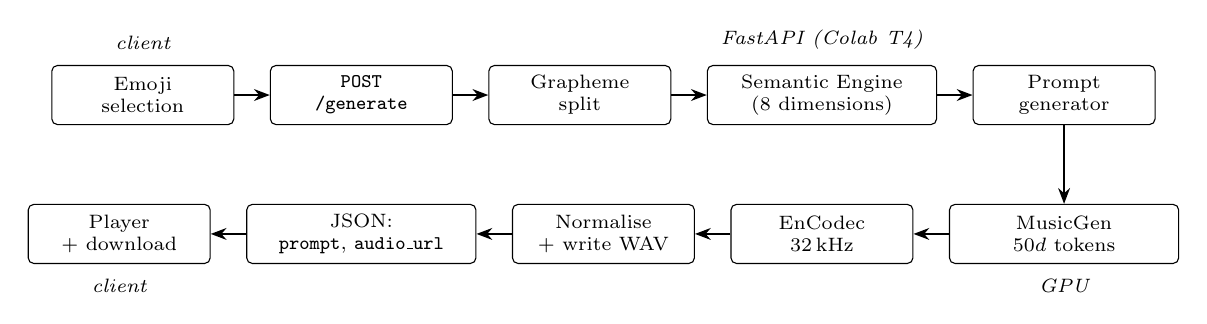
\begin{tikzpicture}[node distance=4.5mm]
  % --- row 1 -----------------------------------------------------------
  \node[box] (sel) {Emoji\\selection};
  \node[box, right=of sel] (post) {\texttt{POST}\\\texttt{/generate}};
  \node[box, right=of post] (split) {Grapheme\\split};
  \node[wide, right=of split] (sem) {Semantic Engine\\(8 dimensions)};
  \node[box, right=of sem] (prm) {Prompt\\generator};

  \draw[arr] (sel) -- (post);
  \draw[arr] (post) -- (split);
  \draw[arr] (split) -- (sem);
  \draw[arr] (sem) -- (prm);

  % --- row 2 (right to left) -------------------------------------------
  \node[wide, below=10mm of prm] (mg) {MusicGen\\$50d$ tokens};
  \node[box, left=of mg] (enc) {EnCodec\\32\,kHz};
  \node[box, left=of enc] (wav) {Normalise\\+ write WAV};
  \node[wide, left=of wav] (json) {JSON:\\\texttt{prompt}, \texttt{audio\_url}};
  \node[box, left=of json] (play) {Player\\+ download};

  \draw[arr] (prm) -- (mg);
  \draw[arr] (mg) -- (enc);
  \draw[arr] (enc) -- (wav);
  \draw[arr] (wav) -- (json);
  \draw[arr] (json) -- (play);

  % --- tier annotations -------------------------------------------------
  \node[lbl, above=1.5mm of sel] {client};
  \node[lbl, above=1.5mm of sem] {FastAPI (Colab T4)};
  \node[lbl, below=1.5mm of play] {client};
  \node[lbl, below=1.5mm of mg] {GPU};
\end{tikzpicture}
\caption{End-to-end generation pipeline. Emoji are converted to structured
attributes and then to text; the model never sees the emoji themselves.}
\label{fig:pipeline}
\end{figure}

The response carries the prompt that was actually used, a relative
\texttt{audio\_url}, the full attribute reading, and a \texttt{meta} block
reporting sample rate, rendered seconds and wall-clock render time. Exposing
\texttt{meta} makes the contract self-diagnosing: a client can compare what
it asked for against what the server produced, which is precisely how the
defect in Section~\ref{sec:numbers} was localised.

% ==========================================================================
\section{Methodology}
% ==========================================================================

\subsection{Representation}
Each emoji is stored as an eight-tuple: \emph{valence} $\in[-1,1]$,
\emph{energy} $\in[0,1]$, \emph{tension} $\in[0,1]$, \emph{hue} (degrees,
used for the interface), \emph{tempo} (BPM), \emph{mode}
(major/minor/modal), an ordered instrument list, and a one-word
\emph{texture}. Valence, energy and tension follow standard dimensional
models of affect; the remaining fields are the musical realisation of that
affect.

\subsection{Fusion}
A selection of $n$ emoji is reduced to one \emph{Reading} (Figure~\ref{fig:fusion}).
Continuous dimensions are averaged,
\begin{equation}
\bar{v}=\frac{1}{n}\sum_{i=1}^{n} v_i,\qquad
\bar{e}=\frac{1}{n}\sum_{i=1}^{n} e_i,\qquad
\bar{t}=\frac{1}{n}\sum_{i=1}^{n} t_i,\qquad
\overline{\text{bpm}}=\mathrm{round}\Big(\tfrac{1}{n}\textstyle\sum_i \text{bpm}_i\Big),
\end{equation}
while \emph{mode} is decided by majority vote, falling back to
\texttt{modal} on a tie --- a deliberate choice, since an unresolved
major/minor split is musically better served by a floating tonality than by
an arbitrary tie-break. Instruments and textures are concatenated in
selection order, de-duplicated, and truncated to 4 and 3 entries
respectively to keep the prompt compact, as MusicGen responds better to a
short description than a paragraph.

Genre is assigned by a six-branch decision over the fused energy--valence
plane; for example $\bar{e}>0.75 \wedge \bar{v}<0.4$ yields
\emph{cinematic electronic}, whereas $\bar{e}<0.35 \wedge \bar{v}<0$ yields
\emph{cinematic ambient}. Continuous $\bar{v}$ and $\bar{e}$ are finally
quantised into five mood words and four energy bands, which supply the
adjectives for the sentence.

\begin{figure}[htbp]
\centering
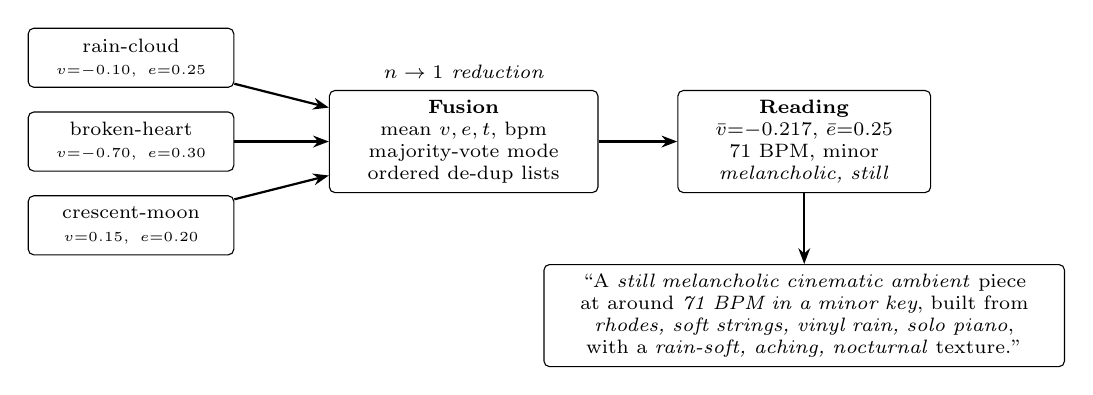
\begin{tikzpicture}[node distance=5mm]
  \node[box, text width=24mm] (e1) {rain-cloud\\{\tiny $v{=}{-}0.10,\ e{=}0.25$}};
  \node[box, text width=24mm, below=3mm of e1] (e2) {broken-heart\\{\tiny $v{=}{-}0.70,\ e{=}0.30$}};
  \node[box, text width=24mm, below=3mm of e2] (e3) {crescent-moon\\{\tiny $v{=}0.15,\ e{=}0.20$}};

  \node[wide, right=12mm of e2, text width=32mm] (fuse)
    {\textbf{Fusion}\\mean $v,e,t,$ bpm\\majority-vote mode\\ordered de-dup lists};

  \node[wide, right=10mm of fuse, text width=30mm] (read)
    {\textbf{Reading}\\$\bar v{=}{-}0.217$, $\bar e{=}0.25$\\$71$ BPM, minor\\\emph{melancholic, still}};

  \node[wide, below=9mm of read, text width=64mm] (txt)
    {``A \emph{still melancholic cinematic ambient} piece at around
      \emph{71 BPM in a minor key}, built from \emph{rhodes, soft strings,
      vinyl rain, solo piano}, with a \emph{rain-soft, aching, nocturnal}
      texture.''};

  \draw[arr] (e1) -- (fuse);
  \draw[arr] (e2) -- (fuse);
  \draw[arr] (e3) -- (fuse);
  \draw[arr] (fuse) -- (read);
  \draw[arr] (read) -- (txt);
  \node[lbl, above=1mm of fuse] {$n \rightarrow 1$ reduction};
\end{tikzpicture}
\caption{Semantic fusion. Three emoji vectors collapse to a single reading,
which is verbalised into one MusicGen prompt. Values shown are the actual
table entries.}
\label{fig:fusion}
\end{figure}

\subsection{Prompt construction}
The generator emits one sentence naming, in order: energy, mood, genre,
tempo, tonality, instrumentation and texture. Fixing this ordering means two
selections that differ in one dimension produce prompts that differ in one
clause, which makes the effect of any single emoji directly observable.

% ==========================================================================
\section{Novelty}
% ==========================================================================

The novelty is interfacial rather than architectural; no model is trained.
Three aspects distinguish the work.

\begin{enumerate}[leftmargin=*, itemsep=2pt, topsep=3pt]
\item \textbf{A compressed conditioning surface.} A 32-emoji palette admits
$2^{32}-1 = 4{,}294{,}967{,}295$ distinct non-empty selections, each mapping
deterministically to a prompt. A very small control vocabulary therefore
addresses a very large descriptive space, without the user writing prose.

\item \textbf{Interpretable, auditable conditioning.} Because fusion is
arithmetic over a published table rather than a learned embedding, every
prompt can be traced to the rows that produced it. Contrast this with feeding
emoji straight to a language model, where the emotion-to-music mapping is
opaque and non-reproducible.

\item \textbf{Separation of affect from realisation.} Valence, energy and
tension are stored independently of tempo, mode and instrumentation. The
affective layer can be re-realised for a different genre or a different
backend model without re-authoring the emotional semantics.
\end{enumerate}

% ==========================================================================
\section{Quantitative Characterisation}
\label{sec:numbers}
% ==========================================================================

Table~\ref{tab:numbers} summarises the deployed configuration. Values are
read from the implementation; latency is a design budget rather than a
benchmarked mean, and is reported as such.

\begin{table}[htbp]
\centering
\small
\caption{Deployed system parameters.}
\label{tab:numbers}
\begin{tabular}{@{}llr@{}}
\toprule
\textbf{Layer} & \textbf{Quantity} & \textbf{Value} \\
\midrule
Palette   & Emoji in backend table            & 32 \\
          & Mood groups                       & 6 \\
          & Dimensions per emoji              & 8 \\
          & Distinct non-empty selections     & $2^{32}-1$ \\
\midrule
Fusion    & Genre decision branches           & 6 \\
          & Mood words / energy bands         & 5 / 4 \\
          & Instrument cap / texture cap      & 4 / 3 \\
\midrule
Model     & Parameters (\texttt{musicgen-small}) & $\approx$300M \\
          & Token frame rate                  & 50\,Hz \\
          & Tokens for 10\,s / 30\,s          & 500 / 1500 \\
          & Guidance scale                    & 3.0 \\
          & Precision / device                & fp16 / T4 16\,GB \\
\midrule
Audio     & Sample rate, depth                & 32\,kHz, PCM-16 \\
          & Peak normalisation                & 0.97 \\
          & Bytes for a 10\,s mono clip       & 640{,}044 \\
          & Server-side retention             & 120\,min \\
\midrule
Client    & Request timeout                   & 180\,s \\
          & Visualiser bands (FFT size 128)   & 64 \\
\bottomrule
\end{tabular}
\end{table}

\paragraph{A worked diagnostic.}
During integration the service returned clips of exactly $0.94$\,s
regardless of the requested duration. Equation~\eqref{eq:tokens} inverts
cleanly: $0.94 \times 50 = 47$ frames, and $47 = 50 - 3$, where three frames
are consumed by the delay pattern across MusicGen's four codebooks. The
observation therefore localises the fault to a generation budget of 50
tokens --- a duration of $1$\,s reaching the model --- rather than to
decoding or file writing. This is a useful property of the design: because
the token--duration relation is exact, an output length is itself a
diagnostic signal. The client now surfaces \texttt{meta.seconds} and warns
whenever the server returns less than half of the requested duration.

\paragraph{A measured coverage defect.}
Comparing the two palettes programmatically showed that the interface and
the backend table have drifted apart. Of the 32 emoji offered by the front
end, only \textbf{14 are present} in the authoritative backend table; the
remaining \textbf{18 (56.3\%)} resolve to the neutral fallback profile
($v{=}0.10$, $e{=}0.45$, modal, piano and pads). Those selections still
produce audio, but the audio is not conditioned on the emotion the user
chose --- a silent failure invisible from the interface. The backend already
exposes a \texttt{/palette} endpoint intended to prevent exactly this, so the
remedy is to drive the front-end grid from that endpoint rather than from a
hard-coded mirror. Table~\ref{tab:coverage} records the current state.

\begin{table}[htbp]
\centering
\small
\caption{Front-end palette coverage against the authoritative backend table.}
\label{tab:coverage}
\begin{tabular}{@{}lrr@{}}
\toprule
\textbf{Status} & \textbf{Count} & \textbf{Share} \\
\midrule
Mapped to a curated profile & 14 & 43.7\,\% \\
Falling back to neutral     & 18 & 56.3\,\% \\
\midrule
Total offered in the interface & 32 & 100\,\% \\
\bottomrule
\end{tabular}
\end{table}

\FloatBarrier

% ==========================================================================
\section{Conclusion}
% ==========================================================================

EmojiMuse demonstrates that a small, hand-authored affective table is
sufficient to drive a text-conditioned music generator from an input as
sparse as a handful of emoji. Keeping the semantic layer explicit --- and
keeping the model strictly downstream of it --- yields a system that is
deterministic, inspectable, and cheap to extend: adding an emoji means adding
one row, not retraining anything.

The quantitative pass proved as valuable as the implementation. The exact
token-to-duration relation turned an opaque truncation into a solved
arithmetic problem, and a direct comparison of the two palettes revealed that
a majority of the interface's controls were not in fact conditioning the
model. Both findings argue the same point: in a multi-stage generative
pipeline, the interfaces between stages deserve the same scrutiny as the
generative stage itself.

Immediate work is to serve the palette from \texttt{/palette} so the two
tables cannot diverge, and to display the server's returned prompt rather
than the client's local approximation of it. Beyond that, the affective layer
is model-agnostic: substituting a larger MusicGen variant, or an LLM that
elaborates the reading into richer prose before conditioning, requires no
change to the emoji semantics.

\end{document}
